\subsection{Introduction}
The Compact Muon Solenoid (CMS)~\cite{CMS:2008xjf} is one of two general-purpose detectors at the LHC. One of the main goals for CMS was the discovery of the Higgs boson, which since its observation in 2012~\cite{CMS:2012qbp,ATLAS:2012yve}, has evolved into a goal of understanding the Higgs boson's properties and assessing their compatibility with the SM. Further motivation for the CMS experiment is the search for physics beyond the Standard Model, like supersymmetry, extra dimensions, and dark matter. These physics goals led to the following priorities for the design of the CMS detector:
\begin{enumerate}
  \item good muon identification and momentum resolution, good dimuon mass resolution, and the ability to unambiguously determine the charge of muons;
  \item good charged-particle momentum resolution and reconstruction efficiency, and efficient triggering and tagging of tau leptons and b-jets, requiring pixel detectors close to the interaction point;
  \item good electromagnetic energy resolution and good diphoton and dielectron mass resolution, as well as efficient $\pi^0$ rejection;
  \item good dijet-mass resolution, and good missing momentum resolution, requiring hermetic geometric coverage.
\end{enumerate}
The centre-of-mass energy provided by the LHC allows CMS to probe physics up to the \TeV scale. Therefore, the detector is designed such that the above requirements should hold for particles with momenta up to 1\TeV. 

Besides its collision energy, the LHC is also unprecedented in its luminosity, with bunch crossings occurring every 25~\unit{ns}, and multiple interactions per bunch crossing. The number of coincident interactions per bunch crossing is referred to as \textit{pileup}, and during the 2015--2018 data taking period, had an average value of 34 at CMS\footnote{An experiment can have a reduced luminosity if desired by choosing to cross the LHC beams with a smaller overlap. Typically, the CMS and ATLAS experiments operate at the maximum possible luminosity whilst the LHCb experiment chooses a lower luminosity that is preferable for measuring b decays.}~\cite{LumiPubl64:online}. This high luminosity environment requires a high level of spatial and timing granularity in the detector, and a fast readout system. Furthermore, high radiation levels are expected, which requires radiation-hard detectors and front-end electronics.

A schematic of the CMS detector is given in \cref{fig:cms_detector}. The structure takes a cylindrical shape, with the beam pipe running through the central axis. The detector is divided into a barrel region, which covers the central region of the detector, and two endcaps, which cover each end of the detector. Key to the design of CMS, is a 13-\unit{m}-long, 6-\unit{m}-inner-diameter, 3.8-\unit{T} superconducting solenoid magnet centred around the beam pipe which provides a high bending power for charged particles which in turn allows for precise momentum measurements. The solenoid envelopes the inner tracker and calorimetry while the muon system is located outside the solenoid, and is embedded in the return yoke of the magnet. 

\begin{figure}
  \centering
  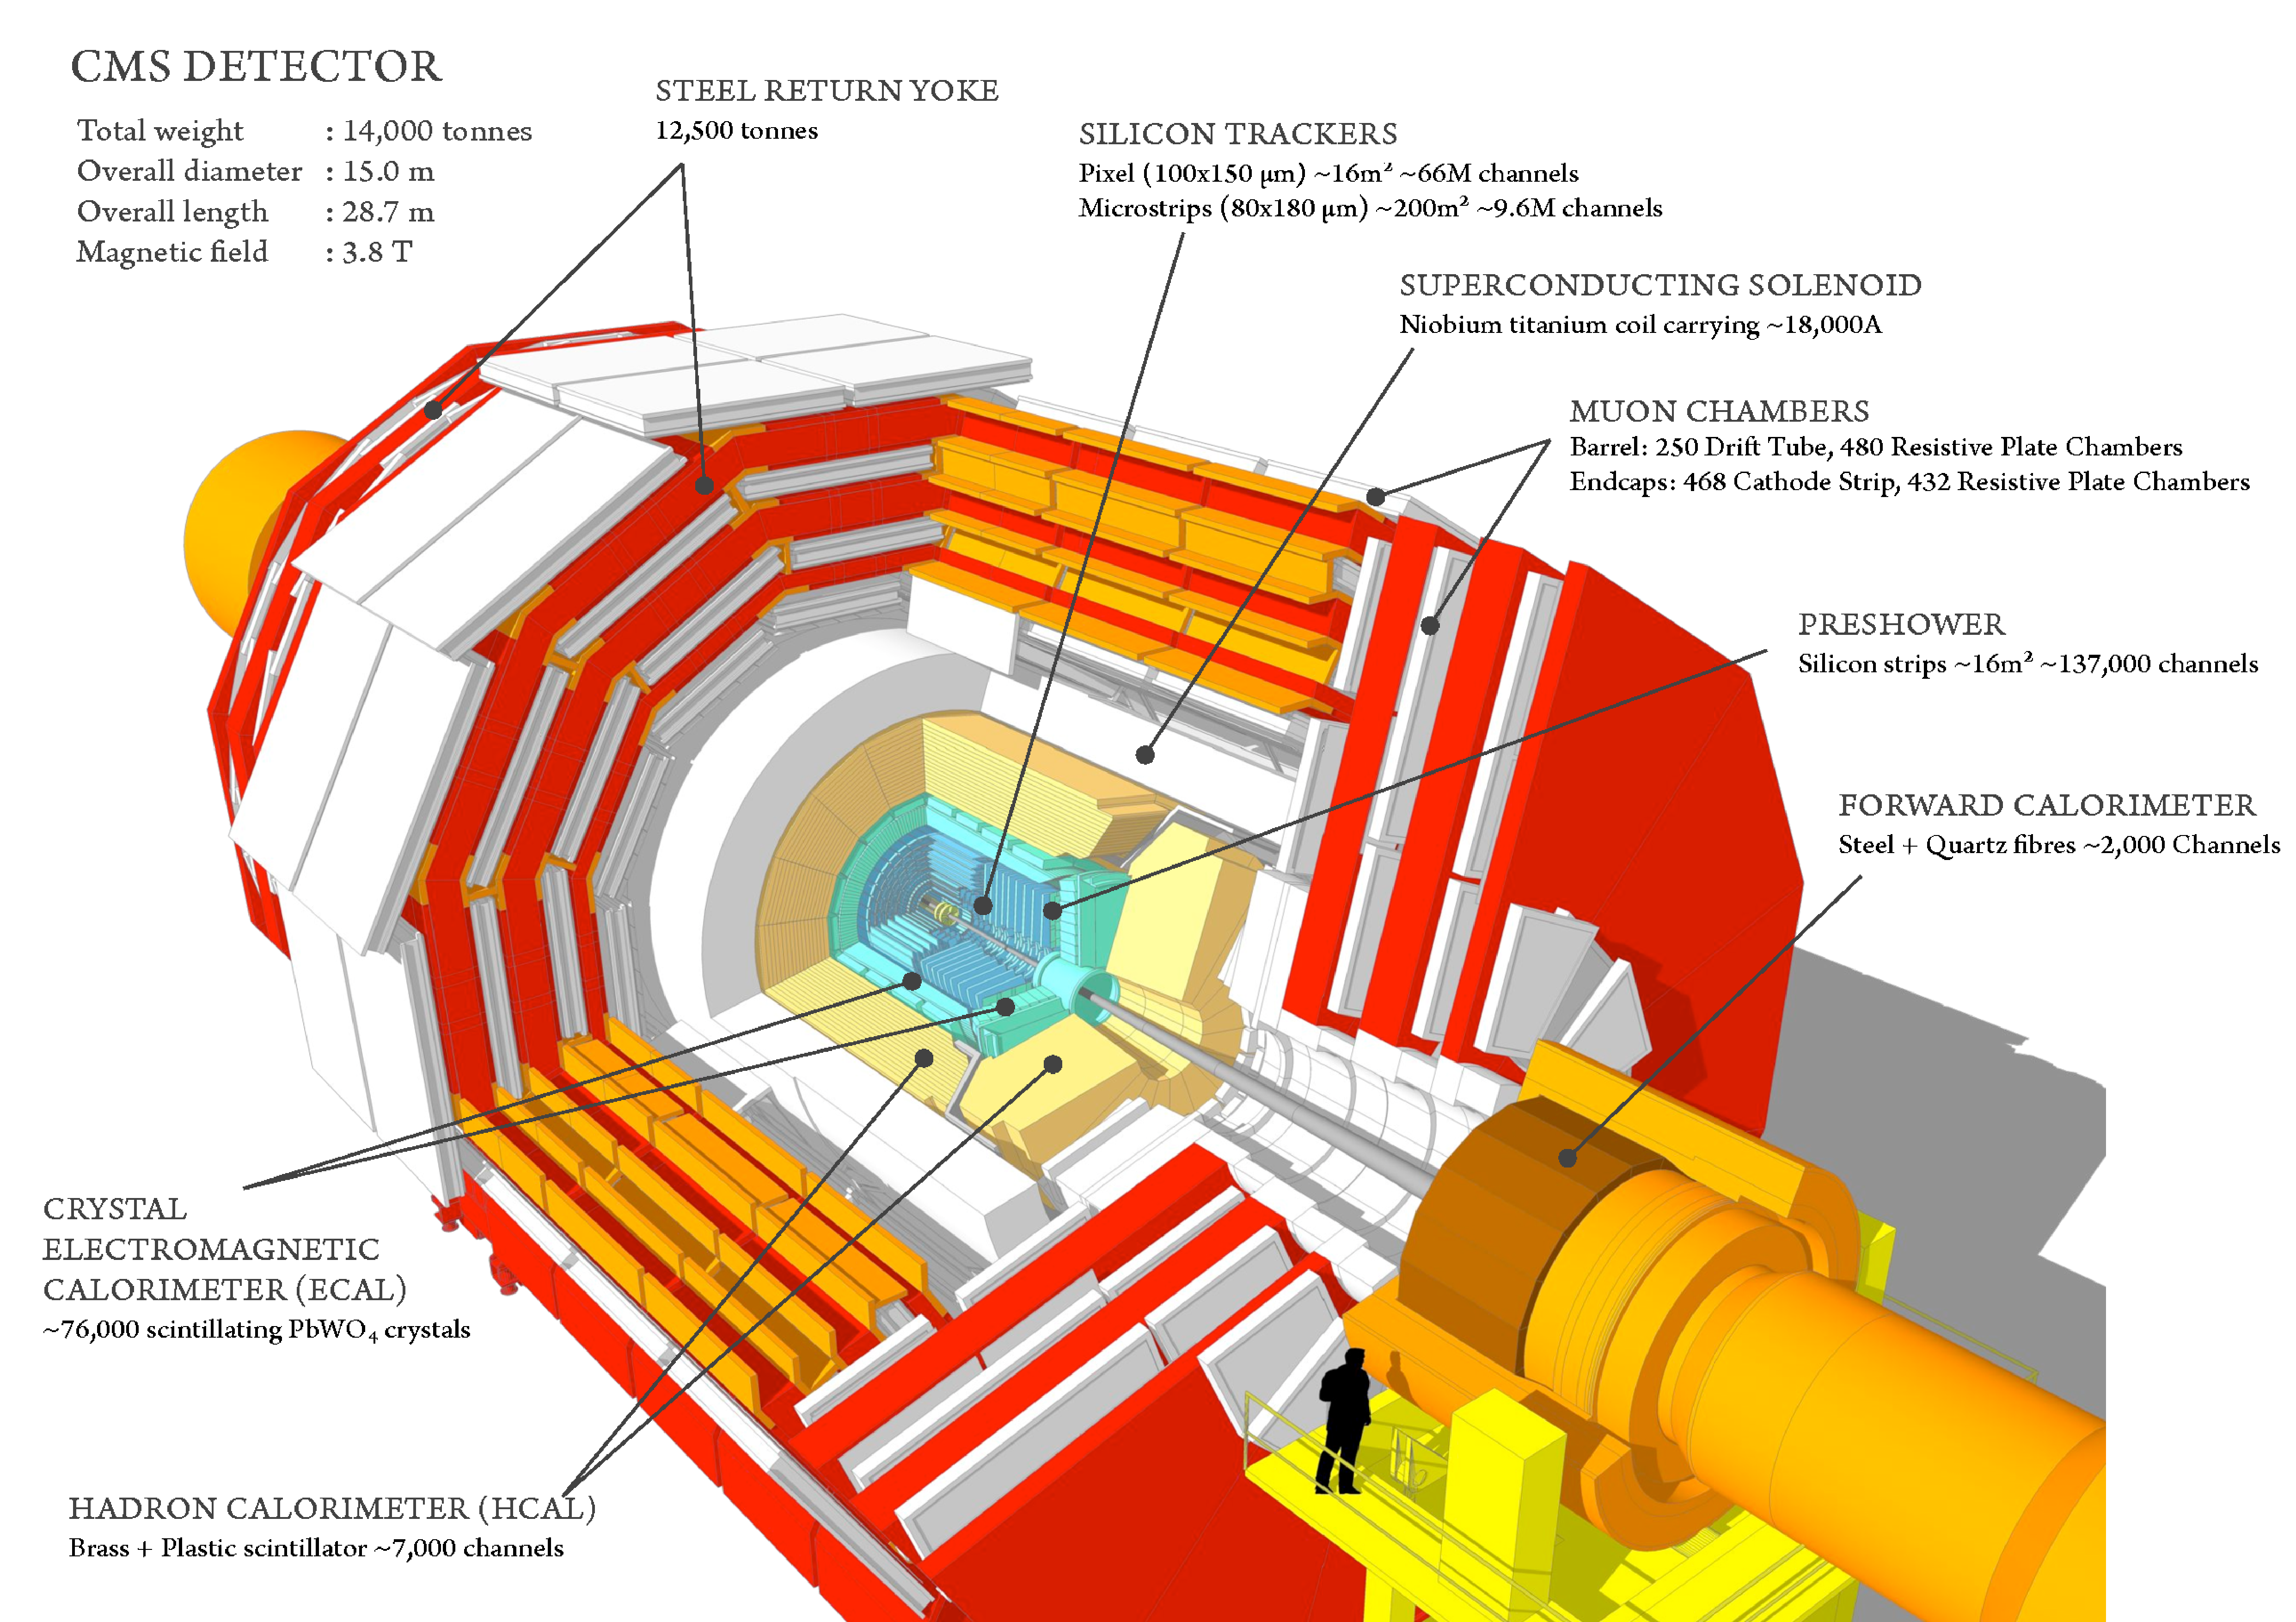
\includegraphics[width=\textwidth]{Figures/Detector/CMS/cms_detector.pdf}
  \caption[A Schematic of the CMS Detector]{A schematic of the CMS detector. Taken from Ref.~\cite{Sakuma:2013jqa}.}\label{fig:cms_detector}
\end{figure}

The di-Higgs search of \cref{chap:dihiggs} uses all key aspects of the CMS detector since it involves the measurements of photons, and the measurement of tau leptons, whose decay products include charged and neutral hadrons, electrons, and muons. In the di-Higgs analysis, good resolution for the diphoton and ditau invariant masses is crucial to separate signal from background, and identify the mass of a new particle, if found. Therefore, the electromagnetic calorimeter (ECAL) and the inner tracker are of particular importance because they determine the energy and momentum of photons and charged particles (majority of tau lepton decay products) respectively.